\input{pre}

\tikzset{rrail/.style={rground,yscale=-1}}
\newcommand{\reffig}[1]{Fig.~\ref{#1}}

\begin{document}
\input{frontpage}
\newpage
\section{Experiment 1}

We measured the dependence of the differential pair currents \(I_1\) and \(I_2\) on the differential input voltage \(\delta V\). The results can be seen in \reffig{fig:ex1}. The linear fits have been done with the values of the currents for \(-0.04 \le V_1-V_2 \le 0.04\), where they present a stronger linearity. The equations are
\begin{align*}
&I_1  = 1.414\cdot10^{-7}(V_1-V_2 )+1.23\cdot10^{-8} \\
&I_2  = -1.406\cdot10^{-7}(V_1-V_2 )+1.18\cdot10^{-8} \\
&I_1+I_2  = 4\cdot10^{-10}(V_1-V_2 )-2.24\cdot10^{-8} \\
&I_1-I_2  = 2.821\cdot10^{-7}(V_1-V_2 )+5\cdot10^{-10}
\end{align*}

From these equations we calculate the offset voltage that makes \(I_1=I_2\) as \(-1.8 mV\). \\

As shown in exercise 5b of the pre-lab, the slope of \(I_1-I_2\) is
\begin{equation*}
g_m = \frac{dI_{out}}{dV_{in}} = \frac{I_b\kappa}{2U_T}
\end{equation*}
%
Assuming that the currents change linearly between 0 and \(I_b\), we can approximate the voltage range in which there is a linear behaviour
\begin{equation*}
\Delta V_{linear} \cdot g_m = I_b
\end{equation*}
\begin{equation*}
\Delta V_{linear} = \frac{I_b}{g_m}=\frac{2U_T}{\kappa}
\end{equation*}
We can see that the linear range is proportional to the thermal voltage, \(U_T\).\\

\begin{figure}
    \center
    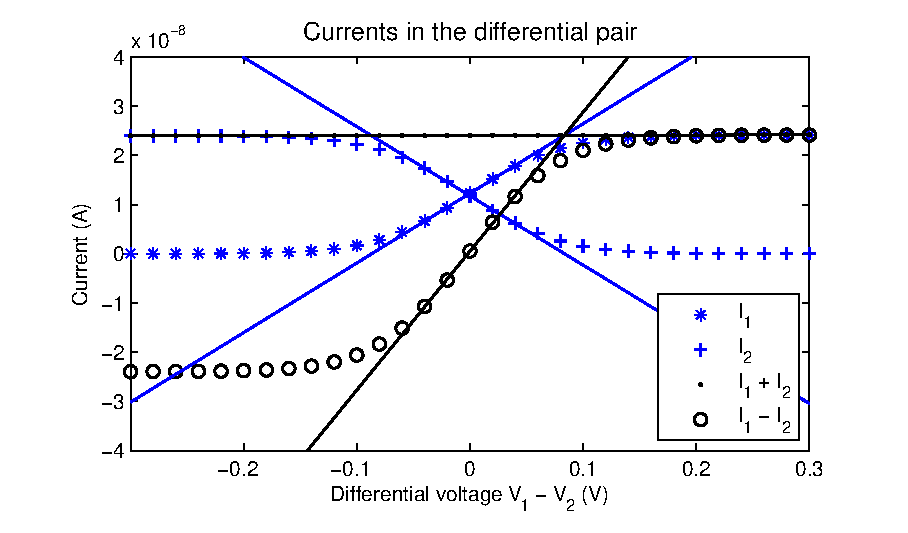
\includegraphics{q1.eps}
    \caption{Currents \(I_1\), \(I_2\), \(I_1+I_2\) and \(I_1-I_2\) in a differential pair as a function of the differential input voltage, \(V_1-V_2\), and their respectives linear fits for small input voltage.}
    \label{fig:ex1}
\end{figure}

If we run the differential pair in strong inversion, we find that the linear range is now proportional to \(V_b\)
\begin{equation*}
g_m = \frac{dI_{out}}{dV_{in}} = \sqrt{\beta I_b}
\end{equation*}
\begin{equation*}
\Delta V_{linear} = \frac{I_b}{g_m}=\sqrt{\frac{I_b}{\beta}} = \sqrt{\frac{k}{2}}(V_b-V_T)
\end{equation*}
\\
\section{Experiment 2}

We now measure the input-output relationship of the bump-antibump circuit. The experimental results can be seen in \reffig{fig:ex2}

\begin{figure}[!htb]
	\center
	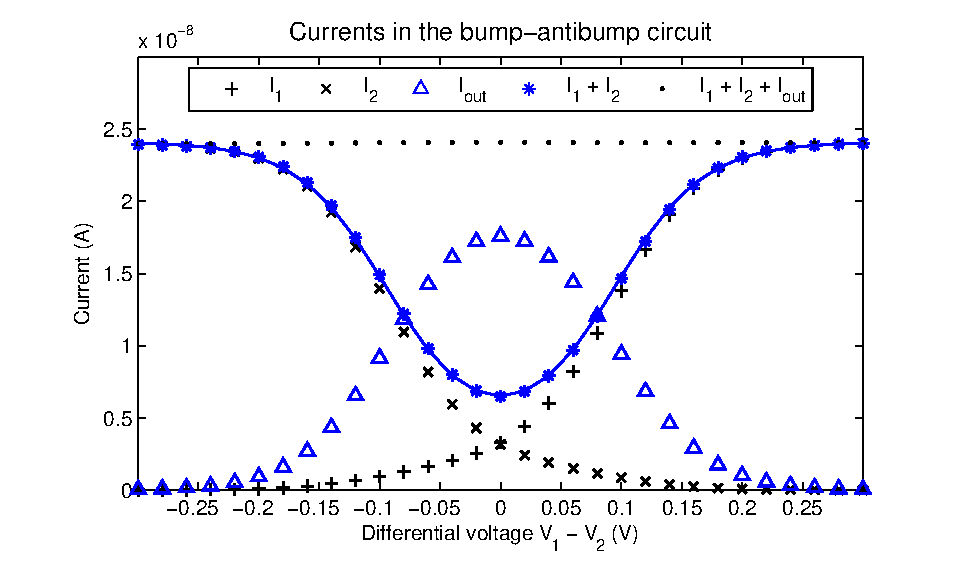
\includegraphics{q2.eps}
	\caption{Currents \(I_1\), \(I_2\), \(I_{out}\), \(I_1+I_2\) and \(I_1+I_2+I_{out}\) in a bump-antibump circuit as a function of the differential input voltage, \(V_1-V_2\). The line corresponds to a non-linear fit of the anti-bump current.}
	\label{fig:ex2}
\end{figure}

From question 4b of the prelab we know that 
\begin{equation*}
I_{anti-bump} = I_b-\frac{I_b}{1+\frac{4}{r}cosh^2(\frac{\kappa \Delta V}{2U_T})}
\end{equation*}
We did a non-linear fit to the experimental data using the model specified by this equation with parameters \(I_b, r, \kappa\) and \(U_T\) and got the following result, which is plotted in the Fig.2:

\begin{equation*}
I_{anti-bump} = 2.41\cdot10^{-8}-\frac{2.41\cdot10^{-8}}{1+\frac{4}{10.8}cosh^2(\frac{0.45 \Delta V}{2\cdot0.033})}
\end{equation*}

When \(V_1=V_2\), the current through the middle branch is given by

\begin{equation*}
I_{out} = \frac{I_b}{\frac{4}{r}+1}
\end{equation*}
where 
\begin{equation*}
r = \frac{\frac{W}{L}\big|_{out}}{\frac{W}{L}\big|_{in}} 
\end{equation*}
According to the specified widths and lengths of the transistors, \(r\) is supposed to be 5 . With this we obtain
\begin{equation*}
I_{out} = \frac{5}{9}I_b=0.56I_b
\end{equation*}
However, we find \(I_{out}\) to be \(0.73I_b\).
If we now use \(r=10.8\) as obtained from the non-linear fit, we get the correct value \(I_{out}=0.73I_b\). \\

The discrepancy in the value of \(r\), which makes \(I_{out}\) larger than expected, can be caused by a short-channel effect. Because the transistors in the middle branch are shorter than those in the side branches and their \(Vds\) is large, they will be more affected by the Early effect and more current will flow through them. 



\end{document}
